\chapter{{Multivariate Cryptography}}

%falar de multivariados em general
\section{Basic Notation}
%Falta corregir hablar de multivariables en general
In the context of multivariate cryptography, we mostly deal with systems of multivariate quadratic polynomials functions over finite fields. In this work, by $\mathbb{F}_q$, or GF($q$) we denote a finite field consisting of $q$ elements, and by $\mathbb{E}$ a extension field of $\mathbb{F}_q$. By $\mathbb{F}_q^n$ we shall denote the vector space of $n$-tuples over $\mathbb{F}_q$. Elements of $\mathbb{F}_q^n$ are denoted by bold characters.

A multivariate quadratic system of polynomials functions with $n$ variables and $m$ equations has the following form
\begin{equation}
p^{(k)}(x_1,x_2,\cdots,x_n) = \sum_{1\leq i \leq j \leq n}\gamma_{i,j}^{(k)} x_i x_j + \sum_{i=1}^{n}\beta^{(k)}_i x_i + \alpha^{(k)}
\label{eq:1}
\end{equation}
where $1\leq k\leq m$ and $\gamma_{i,j}^{(k)}, \beta^{(k)}, \alpha^{(k)} \in \mathbb{F}_q$. If $m=n$ the system is called determined, if $m>n$ the system is called overdetermined and if $m<n$ the system is called undetermined. We call $\gamma_{i,j}^{(k)}, \beta^{(k)}, \alpha^{(k)}$ coefficients and $x_ix_j, x_i$ monomials. The product of a coefficient with  a monomial is called a term. We call a multivariate quadratic system $P$ homogeneous if it not contains linear, nor constants terms.
%Setting $y^{(k)} = p^{(k)}(x_1,x_2,\cdots,x_n) = \sum_{1\leq i \leq j \leq n}\gamma_{i,j}^{(k)} x_i x_j + \sum_{i=1}^{n}\beta^{(k)}_i x_i + \alpha^{(k)}$ we, can express \ref{eq:1} as a set of polynomial functions.

A multivariate quadratic system can be expressed as a set 
\[
P:=\{p^{(1)}, p^{(2)}, p^{(3)}\cdots p^{(m)}\}
\] 
of polynomial functions or in equivalent way as a quadratic map $P\colon \mathbb{F}_q^n \rightarrow \mathbb{F}_q^m$

\begin{equation}
 P=\left(\begin{matrix}
    p^{(1)}(x_1,x_2,\cdots,x_n)  \\
    p^{(2)}(x_1,x_2,\cdots,x_n) \\
    \vdots \\
    p^{(m)} (x_1,x_2,\cdots,x_n) 
   \end{matrix}\right).
\label{eq:maprepresentation}
\end{equation}
\noindent
\textbf{Matrix Representation}.
It is possible to write each polynomial function of \eqref{eq:maprepresentation} $p^{(k)}$ as a matrix-vector product using the upper triangular matrix 

\begin{equation}
 P^{(k)}=\left[\begin{matrix}
   \gamma_{1,1}^{(k)} & \gamma_{1,2}^{(k)} & \gamma_{1,3}^{(k)} & \cdots & \gamma_{1,n}^{(k)} & \beta_{1}^{(k)}\\
  0 & \gamma_{2,2}^{(k)} & \gamma_{2,3}^{(k)} & \cdots & \gamma_{2,n}^{(k)} & \beta_{2}^{(k)}\\
  0 & 0 & \gamma_{3,3}^{(k)} & \cdots & \gamma_{3,n}^{(k)} & \beta_{3}^{(k)}\\
  \vdots &  & \ddots &  & \vdots & \vdots\\  
  0 & 0 & \cdots & 0 & \gamma_{n,n}^{(k)} & \beta_{n}^{(k)}\\
   0 & 0 & \cdots & 0 & 0 & \alpha^{k} 
   \end{matrix}\right]
\label{eq:3}
\end{equation}
and the vector $(x_1,x_2,x_3,\cdots,x_n,1)$ in the following form
\begin{equation}
p^{(k)} = (x_1,x_2,x_3,\cdots,x_n,1) P^{(k)} (x_1,x_2,x_3,\cdots,x_n,1)^{T}
\end{equation}

Although, this construction seems strange this will be useful at the chapter \ref{chapter:mpqc} when, we talked about Attacks on Multivariate Quadratic Schemes.

\section{The Standard (Bipolar) Construction}
The standard and most popular construction of multivariate cryptography consists of select a map $P\colon\mathbb{F}_q^{n}\rightarrow \mathbb{F}_q^{m}$ of polynomials functions of degree two as \eqref{eq:maprepresentation}, such that it is easy to find pre-images. Besides, chooses two affine transformations $S\colon\mathbb{F}_q^{m}\rightarrow \mathbb{F}_q^{m}$ and $T\colon\mathbb{F}_q^{n}\rightarrow \mathbb{F}_q^{n}$. These objects are used to construct encryption and signature schemes and we will see that for encryption is necessary that $m\geq n$ and for signature is necessary that $m\leq n$. The public key is the composition $\bar{P} = S \circ P \circ T$ and the private key consists of $S$, $P$ and $T$.\\
\noindent
\textbf{Encryption Schemes}\\
\noindent
\textit{Encryption.} To encrypt a message $\boldsymbol{m}$, it is only necessary compute $\boldsymbol{c} = \bar{P}(\boldsymbol{m})$. The ciphertext of the message $\boldsymbol{m}$ is $\boldsymbol{c}$.\\
\noindent
\textit{Decryption.} To decrypt the ciphertext $\boldsymbol{c}$ is necessary compute $\boldsymbol{y} = S^{-1}(\boldsymbol{c})$, $\boldsymbol{y'} = \bar{P}^{-1}(\boldsymbol{y})$ and the original message is $\boldsymbol{m} = T^{-1}(\boldsymbol{y'})$. Note that $P^{-1}$ do not denote the inverse functions, which might not even exist, but some pre-image. In other words, sometimes is possible to exist another pre-images $\boldsymbol{m_1}, \boldsymbol{m_2}, \cdots \boldsymbol{m_k}$ such that $\bar{P}(\boldsymbol{m_1}) = \bar{P}(\boldsymbol{m_2}) = \cdots = \bar{P}(\boldsymbol{m_k}) = \bar{P}(\boldsymbol{m})$. This problem has been discussed by \cite{Patarin1996} and he suggest to use error correcting codes or hash function to solve it. 

We say that for encryption is necessary that $m\geq n$ because in this case with high probability there is a unique pre-image of $\boldsymbol{y}$ under $\bar{P}$.\\
\noindent
\textbf{Signature Schemes}\\
\noindent
\textit{Signature Generation.} To sign a document $d$, we calculate $\boldsymbol{h} = H(d)$ where $H$ is a hash function. Then we compute $\boldsymbol{y} = S^{-1}(\boldsymbol{h})$, $\boldsymbol{y'} = \bar{P}^{-1}(\boldsymbol{y})$ and the signature of $\boldsymbol{h}$ is $\boldsymbol{z} = T^{-1}(\boldsymbol{y'})$. Again, note that $P^{-1}$ do not denote the inverse functions, which might not even exist, but any pre-image. 

We say that for signature $n \geq m$ because thus we can be sure that such a pre-image exists.
Thus, every message has a signature.\\
\noindent
\textit{Signature Verification.} To verify the  signature $\boldsymbol{z}$ of the document $d$, we compute $P(\boldsymbol{z})$ if the result equal to $\boldsymbol{h}$ the signature is accepted, otherwise it is rejected.\\
\noindent\\
\noindent
\cite{Schneier1995} argued that the use of  hash functions in cryptography schemes 
is that in practical implementations, public-key algorithms are often too inefficient to sign long documents. Thus, to save time, digital signature protocols are often implemented with hash functions. Also, hash functions are used to decrease any pattern or any known structure of a message to sign. 

The security of bipolar constructions is based on the MQ-Problem and IP-Problem problems. The MQ-Problem is proved NP-Complete but not the IP-problem, this fact difficult to construct provable security schemes based on multivariate quadratic systems.
\subsection{Example}
We shall give an example of a standard construction namely Random Singular Simultaneous Equation (R(S)SE) which was proposed by \citet{KasaharaS04}. The reason to chose this is that its simplicity for construction.\\\\
%that is a variation of the scheme  STS proposed by \cite{Tsujii1985}
\noindent
\textit{Key Generation.} The map $P$ in R(S)SE has $L$ layers of polynomials functions. Let $i$ be a $i^{th}$ layer. Each layer has $r_i$ new variables and $m_i$ equations. The $r_i$ values are such that $\sum_{i=1}^{L}r_i=n$ and the $m_i$ values are such that $\sum_{i=1}^{L}r_i=m$. In Figure \ref{fig:RSSE}, we depict the form of the map $P$ for the R(S)SE scheme. 

The public key $\bar{P}$ is constructed by using two affine transformations  $S\colon\mathbb{F}_q^{m}\rightarrow \mathbb{F}_q^{m}$ and $T\colon\mathbb{F}_q^{n}\rightarrow \mathbb{F}_q^{n}$. These two transformations are operated with $\bar{P}$ in the following way $\bar{P} = S \circ P \circ T$. The private key consists of $S$, $P$ and $T$.\\
\noindent
\textit{Encryption.} To encrypt a message $\boldsymbol m$ we only has to evaluate this message in the map $\bar{P}$, i.e. the ciphertext $\boldsymbol c = \bar{P}(\boldsymbol m)$.\\
\noindent
\textit{Decryption.} To decrypt the ciphertext $\boldsymbol c$, we first apply the inverse of the affine transformation $T$ in $\boldsymbol c$. i.e. $\boldsymbol y = T^{-1}(\boldsymbol c)$. After that, we must, to find the pre-image $\boldsymbol x$ of the system $\boldsymbol y = P(\boldsymbol x)$. To calculate the pre-image we need to construct $L$ sub-systems. The left side of each sub-systems has the form as each layer of Figure \ref{fig:RSSE}. To calculate the right side of each sub-system we need to split $\boldsymbol y$ in $L$ layers $\boldsymbol y_1, \boldsymbol y_1, \cdots \boldsymbol y_L$. Each layer $\boldsymbol y_1, \boldsymbol y_1, \cdots \boldsymbol y_L$ has $m_1, m_2, \cdots, m_L$ elements respectively. For the Layer 1, we must compute an vector of variables $\boldsymbol x_1$ for the given vector $\boldsymbol y_1$ such that $\boldsymbol x_1$ has $r_1$ entries. To compute $\boldsymbol x_1$, we need to use brute force, that is, to  compute $\boldsymbol x_1$ it is necessary to make $q^{r_1}$ attempts. After one, we compute a vector of variables $\boldsymbol x_2$ for the given vector $\boldsymbol y_2$ such that $\boldsymbol x_2$ has $r_2$ entries. Again, to compute $\boldsymbol x_2$ we must, to use brute force, that is, to compute $\boldsymbol x_2$ it is necessary to make $q^{r_2}$ attempts. These steps are repeated until we calculate the last vector of variables $\boldsymbol x_L$ with $r_L$ variables. Note, that following the construction of R(S)SE, we are finding $r_i$ new variables in each step. Putting all $\boldsymbol x_i$ together in $x$ we retrieve the original message setting $\boldsymbol m = S^{-1}(\boldsymbol x)$. Note, that in order to obtain a practical scheme the value of $r$ must be small, otherwise a legitimate user has a workload to decrypt.

\begin{figure}
\footnotesize
\[
 P=\left(\begin{array}{l}
 \text{Layer 1}  \left\{\begin{array}{l}
    p^{(1)}(x_1,x_2,\cdots,x_{r_1})  \\
    \quad\quad\vdots\\
    p^{(m_1)}(x_1,x_2,\cdots,x_{r_1})
    \end{array}
    \right.%%%%%%%%%%%%%
    \\
 \text{Layer 2}   \left\{\begin{array}{l}
    p^{(m_1+1)}(x_1,x_2,\cdots,x_{r_1}, x_{r_1+1},x_{r_1+2},\cdots,x_{r_2})  \\
    \quad\quad\vdots\\
    p^{(m_1+m_2)}(x_1,x_2,\cdots,x_{r_1}, x_{r_1+1},x_{r_1+2},\cdots,x_{r_2}) 
     \end{array}
    \right.%%%%%%%%%%%%
   \\
   \quad\quad\quad\quad\quad \quad\quad\quad\quad\quad \vdots\\
 \text{Layer L}   \left\{\begin{array}{l}
   p^{\left(m_{L-1}+1\right)}(x_1,\cdots,x_{r_1}, x_{r_1+1},\cdots,x_{r_2},\cdots, x_{n_{L-1}+1}, \cdots, x_{n_{L-1}+n_L})  \\
    \quad\quad\vdots\\
    p^{(m_{L-1}+m_L)}(x_1,\cdots,x_{r_1}, x_{r_1+1},\cdots,x_{r_2},\cdots, x_{n_{L-1}+1}, \cdots, x_{n_{L-1}+n_L}) \\
   \end{array}\right.
   \end{array}
   \right)
\]
\caption{map $P$ of (R(S)SE)}
\label{fig:RSSE}
\end{figure}
\section{The MQ Problem}
 
As we said, the security of multivariate quadratic schemes relies on the computational hardness of solving large multivariate systems. This problem, called here, the MQ-problem is enunciated as follow. \\
\\
\noindent
\textbf{MQ-Problem.} Given a system $P=\left(p^{(1)}),\cdots, p^{(m)}\right)$ of $m$ non-linear polynomials functions in the variables $x_1,\cdots, x_n$. Is there some $\overline{x_1}, \cdots, \overline{x_n}$ such that $p^{(1)}(x_1,\cdots, x_n)=0, \cdots, p^{(m)}(x_1,\cdots, x_n) = 0$?\\
\\
\noindent
Even for the case of non-linear polynomial functions of degree 2, this problem is proved NP-complete. To show that, it is necessary to reduce the 3-CNF-SAT Problem to the MQ-Problem. A proof of this reduction can be found in the thesis of \cite{wolfphdthesis}. 
\section{Attacks against Multivariate Schemes}
%This section can be complemented with the Section 8.2 in the page 249
There are several attacks which are possible to apply against multivariate schemes. Depending on which of the following problems them trying to solve, \cite{wolfphdthesis} classify these attacks in two types.\\
\noindent
\textbf{Inversion Problem.} Given $(\boldsymbol{x},\boldsymbol{y}) \in \mathbb{F}^n\times \mathbb{F}^m$ a pair message/ciphertext or signature/message and $\bar{P}$ a public key for a multivariate scheme. Recover $\boldsymbol{x}$ for given $\boldsymbol{y}$ and public key $\bar{P}\colon\mathbb{F}_q^{n}\rightarrow \mathbb{F}_q^{m}$.\\
\noindent
Note that the Inversion Problem is the same of the MQ-Problem.\\
\noindent 
\textbf{Key Recovery Problem.} Recover the private key $(S,P,T)$ for a given public key $\bar{P}.$ 

The Inversion Problem plays a important role for the goals of our thesis. Remember that one of our goals is select a set of multivariate schemes together with the known best attack of each one of them. After that, we will fix several security levels against the known best attack of each one. At each level we will compare them to determine who is more resistant to inversion attack using SAT solvers. 
 
We will dealing with the known best attack of each multivariate scheme that are still unbroken in the chapter \ref{chapter:back_ground_mpqc}. In this section, we will describe some general inversion attacks which works against any multivariate schemes. 


%Among them, there is  the Minrank attack proposed by against the multivariate proposed by and called HFE.

\subsection{SAT Solving Attack}

A approach for trying to solve the Inversion Problem is to use SAT solvers. The inversion problem is equivalent to the 3-CNF-SAT problem enunciated in the chapter \ref{chap:satisfiability}. Therefore, it is possible to translate the a system of multivariate polynomials functions into a logical expression in CNF. This 3-CNF-SAT instance is submitted to a SAT solver. [BARD] shows techniques for to make this translating. 

Below, we will describe how to convert instances of the Inversion Problem to the 3-CNF-SAT Problem, using mainly the techniques of [BARD] as reference.


\subsection{Fault Attacks}

[France paper]
\subsection{Groebner Basis Attack}

In this section we will review and to make a theoretical study of the number of equations that determined, undetermined and overdetermined random multivariate quadratic systems should have, to resists attacks from the HybridF5 Algorithm, which is the fastest algorithm to solve them. Basically, this algorithm consists in guess some variables of a multivariate nonlinear equation before to solve it with the F5 algorithm. Guessing variables reduces the complexity of the F5 algorithm, but also increases the number of its runs. 
%Question how many guessing variables?
%to build overdetermined systems
The complexity of solving a system of $m$ quadratic equations in $n$ variables over a finite field with $q$ elements by the HybridF5 algorithm is given by

\begin{equation}
 \text{complexity}_{\text{HF5}}(q,m,n)= \left(\min_{k\geq 0}q^{k}\cdot O\left(m\cdot \binom {n-k+d_{\text{reg}}-1} {d_{\text{reg}}}\right)\right)^\omega
 \label{eq:complexityHF5}
\end{equation}
where, for random systems, the degree of regularity $d_{\text{reg}}$ is given as the lowest integer $D$ for which the coefficient of $t^D$ in $\dfrac{(1-t^2)^m}{(1-t)^n}$ is less or equal to 0 and $2 < \omega \leq 3$ denotes the linear algebra constant of solving a linear system.
Unfortunately, the details of the F5 algorithm are not publicly known, which makes it difficult to estimate the concrete running time the algorithm needs to solve a multivariate system. To derive secure parameters for multivariate schemes from formula \eqref{eq:complexityHF5}, we follow the approach of the thesis of \cite{AlbrechtPetzoldt2013}. He set $\omega = 2$ and get by 
\begin{equation}
 \text{lower bound}_{\text{HF5}}(q,m,n)= \left(\min_{k\geq 0}q^{k}\cdot O\left(m\cdot \binom {n-k+d_{\text{reg}}-1} {d_{\text{reg}}}\right)\right)^2
\label{eq:complexityHF5w}
\end{equation}
a lower bound of the complexity of the HybridF5 algorithm. If this lower bound is larger than the security level, we can be sure that an attack against the multivariate quadratic system with the HybridF5 algorithm is infeasible.

The number of variables $n$ and equations $m$ of this review and study is focused on the selected schemes. The results of this study helps to calculate the parameters of the different selected multivariate quadratic schemes to resist attacks of the HybridF5 algorithm. Different sets of parameters, for each multivariate quadratic scheme, generate several security levels. We will use these sets of parameters to estimate the running time that the SAT solver takes, when it is used to attack multivariate quadratic schemes. All this analysis is in the chapter.

When the system is only slightly undetermined $(m<n<2m)$, then the best strategy to solve it is by fixing $n-m$ of the variables and trying to solve the generated determined system with the HybridF5 algorithm. One can expect that the determined system will have exactly one solution. So the complexity of solving an undetermined system with $m$ equations in $n (m<n<2m)$ variables is the same as that of a determined system with $m$ equations. As was developed by \cite{AlbrechtPetzoldt2013} is his Phd thesis this strategy is applied to attack Rainbow and UOV schemes.
%%%%%%%%% juaninf 20/06/2016
If the system is highly underdetermined system, namely $n\geq m\cdot(m+1)$ \cite{Kipnis1999} found that it can be solved in polynomial time. \cite{Thomae2012} revisiting the Kipnis and Shamir attack found that, when $n = \omega \cdot m$ holds, then the undetermined system of $m$ equations in $n$ variables is hard to solve as a determined system in $m' = m - \lfloor{\omega\rfloor} + 1$ equations. The strategy of fixing $n-m$ of the variables together the improved of \cite{Thomae2012} are taken into account by \cite{AlbrechtPetzoldt2013} when analyse UOV.

For the case of overdetermined system \cite{Kipnis1999} found that if the number of equations and variables is such that $m \geq n(n - 1)/2$ then the system can be solved in polynomial time. In this thesis we have selected the ABC scheme proposed \citep{Tao2013} which has $m=2n$ equations.

\subsubsection{Reviewing the number of equations to solve undetermined systems}

Because the strategy of fixing $n-m$ is better when the HybridF5 algorithm is used against undetermined systems, i.e translate the undetermined system to determined system, \citet{AlbrechtPetzoldt2013} make a theoretical and experimental study of the use of HybridF5 algorithm to solve random determined multivariate quadratic systems. With this study they calculates secure parameters for UOV and Rainbow.

After the fixing strategy, he calculates the number of variables for guessing to build overdetermined systems such that HybridF5 algorithm has better performance. He found:
\begin{itemize}
\item for determined systems over $\mathbb{F}_{16}$ it is the best strategy to guess $5$ ($m \leq 29$), $6$ ($30 \leq m \leq 40$) or $7$ ($m \geq 41$) variables,
\item for determined systems over $\mathbb{F}_{31}$ it is the best strategy to guess $2$ ($m \leq 27$), $3$ ($28 \leq m \leq 35$) or $4$ ($m \geq 36$) variables and
\item for determined systems over $\mathbb{F}_{256}$ it is the best strategy to guess $1$ ($m \leq 32$) or $2$ ($m \geq 33$) variables.
\end{itemize}

With these guessing variables and evaluating equation \eqref{eq:complexityHF5w} for $m\in \left\{20,\cdots, 60\right\}$, he found that the bit complexity of solving a determined random system of $m$ multivariate quadratic equations using the HybridF5 algorithm is roughly
\begin{equation}
2.30 \cdot m + 14.4
\label{eq:complexdetermined_gf16}
\end{equation}
for systems over $\mathbb{F}_{16}$,
\begin{equation}
2.50 \cdot m + 13.0
\label{eq:complexdetermined_gf31}
\end{equation}
for systems over $\mathbb{F}_{31}$ and
\begin{equation}
2.65 \cdot m + 12.1
\label{eq:complexdetermined_gf256}
\end{equation}
for systems over $\mathbb{F}_{256}$.

Besides, the theoretical equations \eqref{eq:complexdetermined_gf16}, \eqref{eq:complexdetermined_gf31} and \eqref{eq:complexdetermined_gf256} he carried out a large number of computer experiments. For these experiments he used MAGMA v. 2.13-10 which contains an efficient implementation of Faugeres F4 algorithm. Although MAGMA v. 2.13-10
was already released in 2008, it is still one of the fastest publicly available solvers for multivariate nonlinear systems and in fact often faster than newer versions of MAGMA. The results of the experiments are very similar to the result of together with the theoretical study.
\subsubsection{Calculating the number of equations to solve overdetermined systems}
\label{subsection:hybridF5overdetermined}
 Next, we are going to compute the number of equations to protect overdetermined random multivariate quadratic systems for the case $m=2\cdot n$, using the complexity of the HybridF5 algorithm.

As \cite{AlbrechtPetzoldt2013}, we use the equation \eqref{eq:complexityHF5w} to compute the complexity of solving overdetermined random systems over $\mathbb{F}_2$, $\mathbb{F}_4$, $\mathbb{F}_{16}$ and $\mathbb{F}_{256}$ with the HybridF5 algorithm when guessing different number of variables. Figures \ref{fig:overgf2}, \ref{fig:overgf4}, \ref{fig:overgf16} and \ref{fig:overgf256} show the results. 

\begin{figure}
\centering
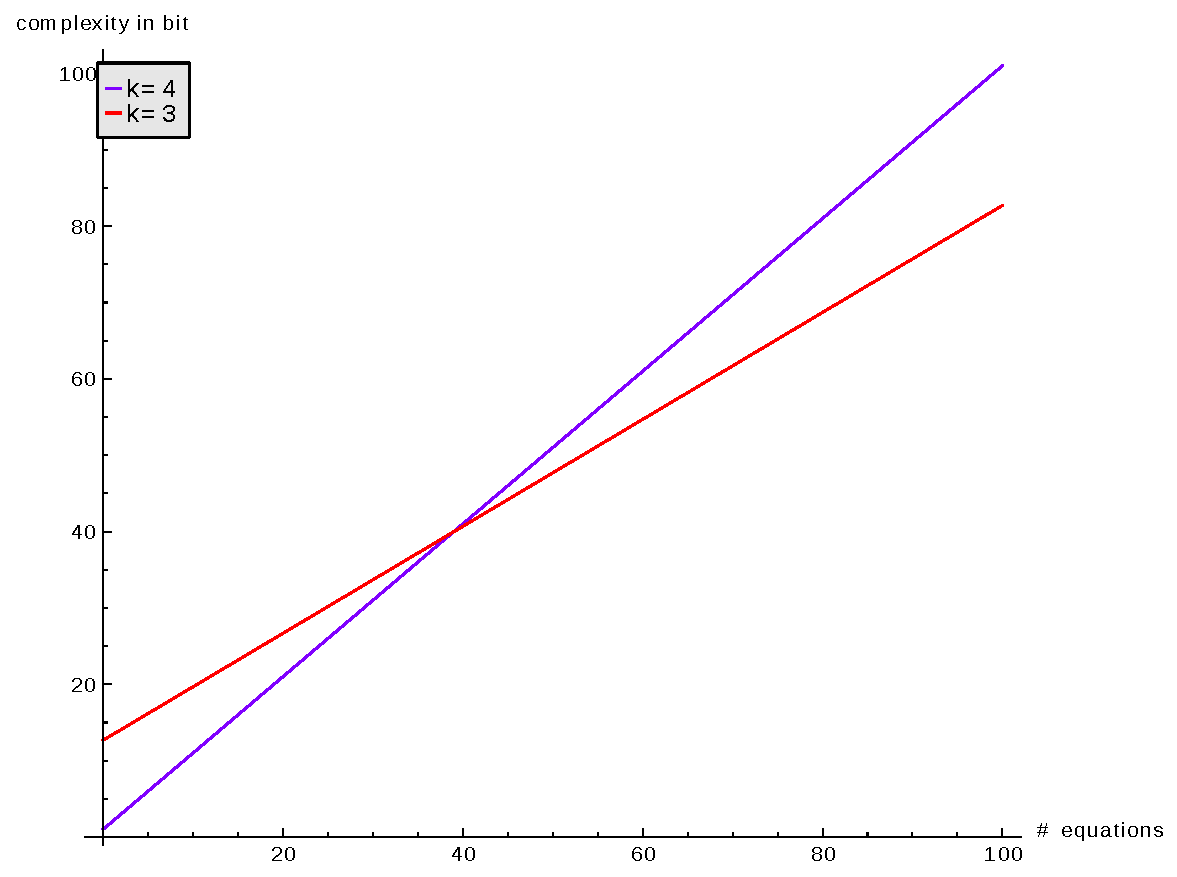
\includegraphics[width=10cm]{figures/hybridF5_vs_m_gf2.pdf}
\caption{Complexity of solving overdetermined random systems over $\mathbb{F}_2$ with HybridF5}
\label{fig:overgf2}
\end{figure}

\begin{figure}
\centering
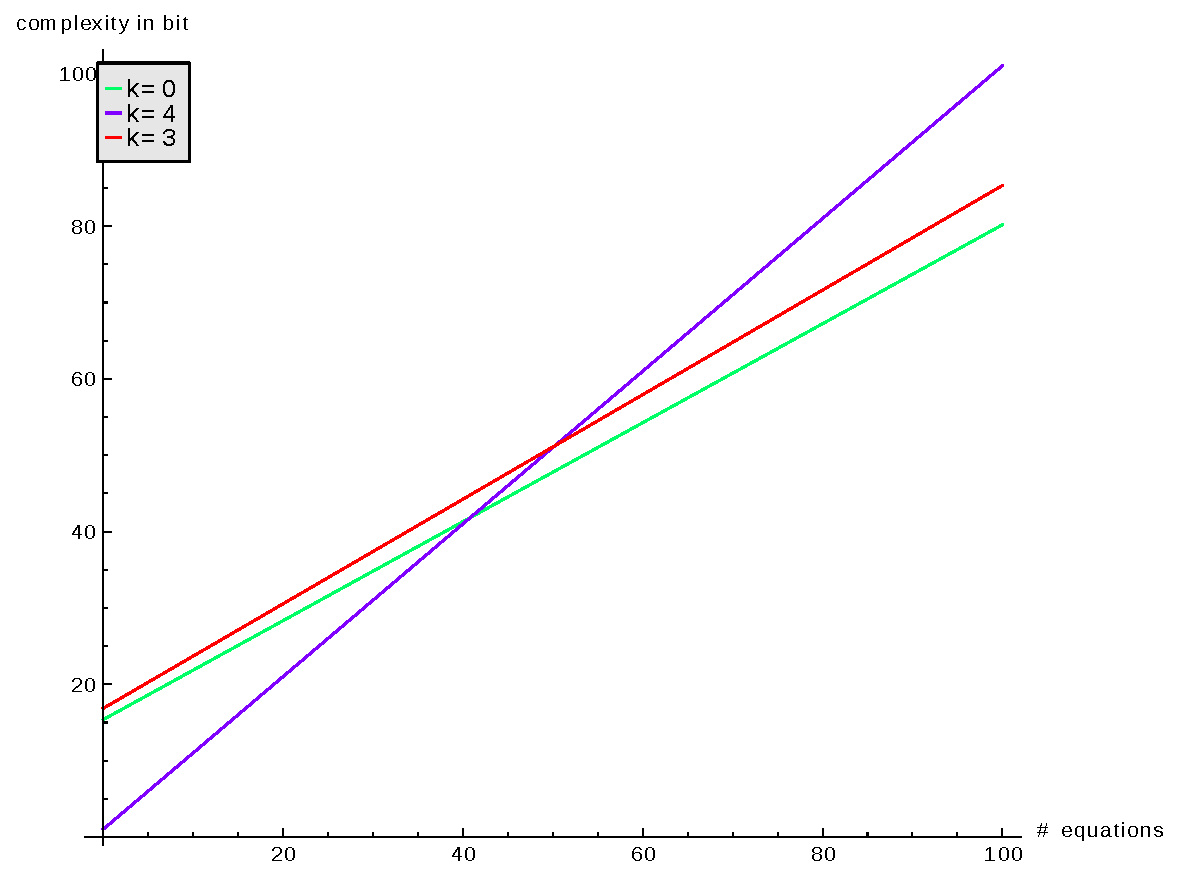
\includegraphics[width=10cm]{figures/hybridF5_vs_m_gf4.pdf}
\caption{Complexity of solving overdetermined random systems over $\mathbb{F}_4$ with HybridF5}
\label{fig:overgf4}
\end{figure}

\begin{figure}
\centering
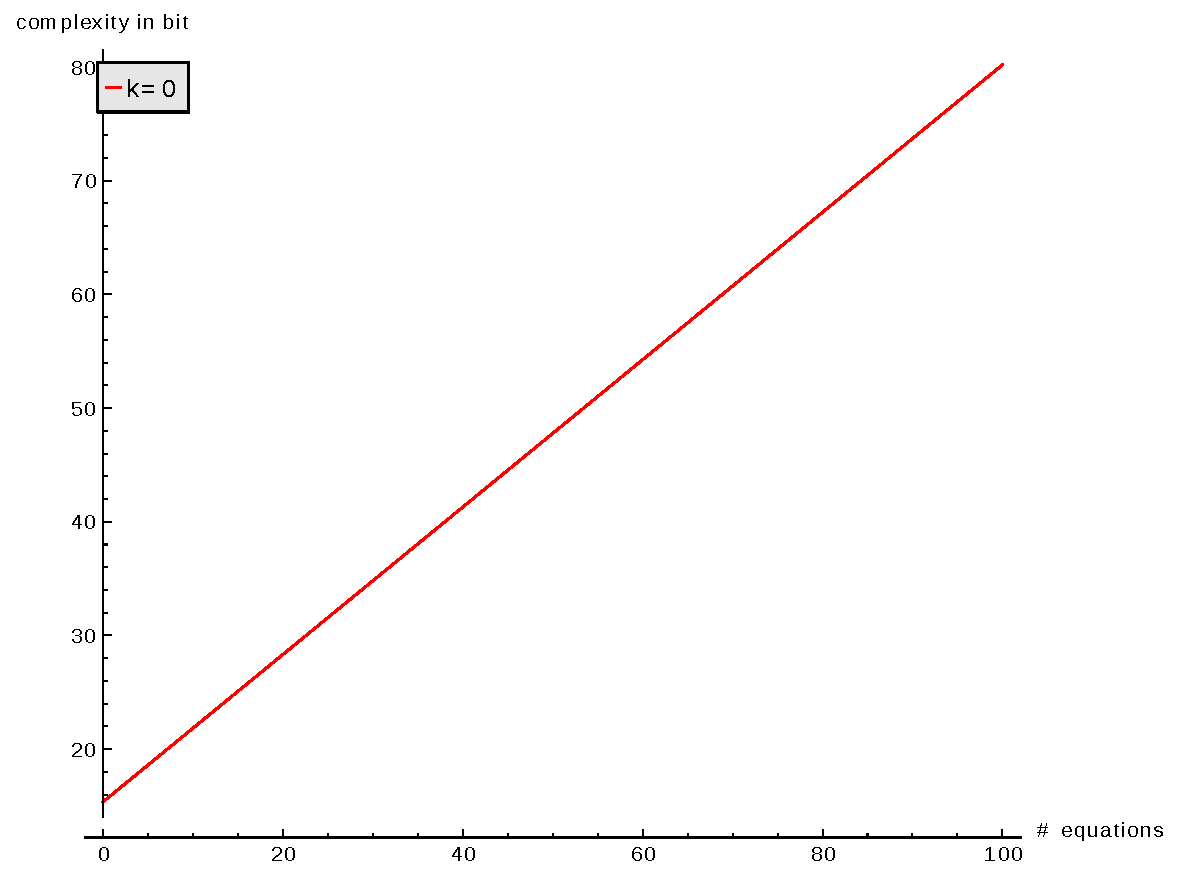
\includegraphics[width=10cm]{figures/hybridF5_vs_m_gf16.pdf}
\caption{Complexity of solving overdetermined random systems over $\mathbb{F}_{16}$ with HybridF5}
\label{fig:overgf16}
\end{figure}


\begin{figure}
\centering
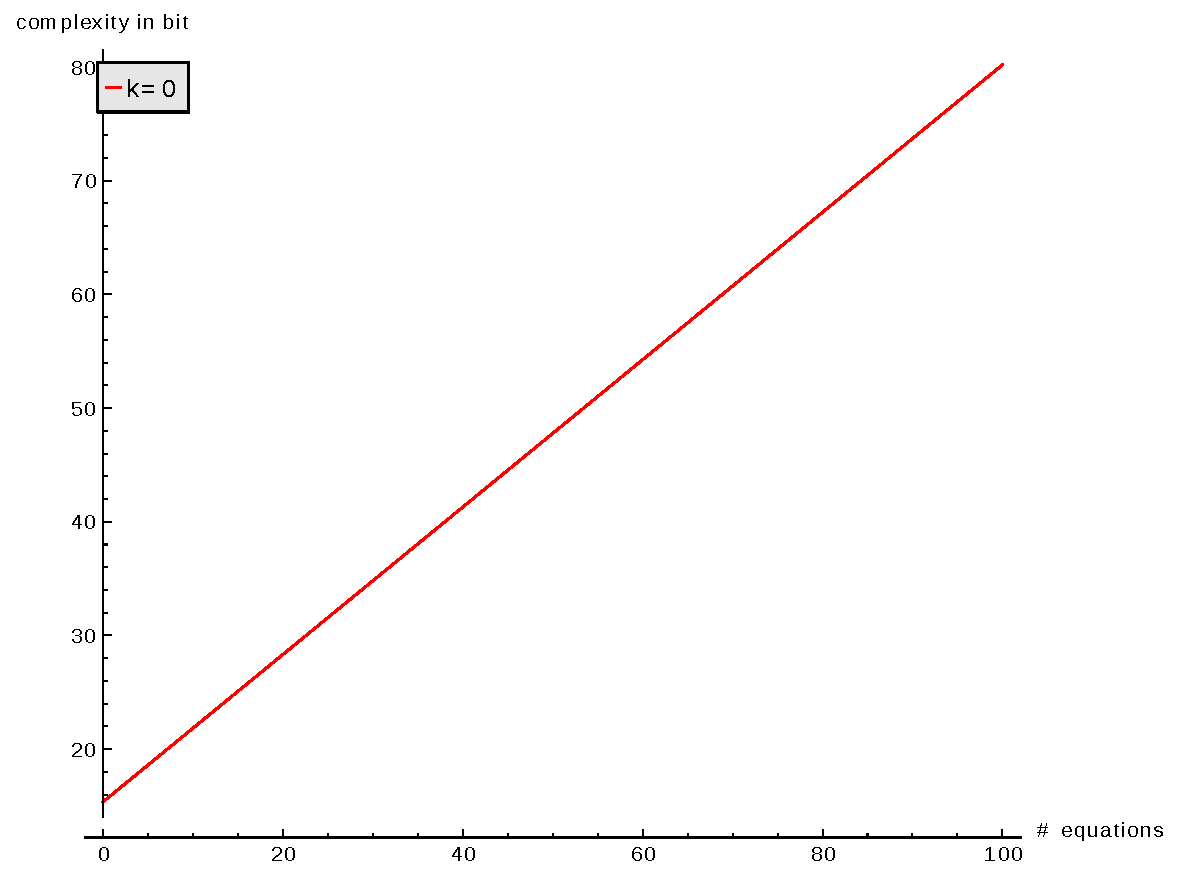
\includegraphics[width=10cm]{figures/hybridF5_vs_m_gf256.pdf}
\caption{Complexity of solving overdetermined random systems over $\mathbb{F}_{256}$ with HybridF5}
\label{fig:overgf256}
\end{figure}
A natural question in this context is to choose the best tradeoff, i.e. for which number $k\geq 0$ the complexity of the algorithm as shown by equation \eqref{eq:complexityHF5w} gets minimal. Guessing variables to build \textbf{overdetermined systems} reduces the complexity of each run of the F5 algorithm, but also increases the number of this runs. We found

\begin{itemize}
\item for overdetermined systems over $\mathbb{F}_{2}$ it is the best strategy to guess $7$ ($m\leq 41$), $6$ ($m\geq 42$),
\item for overdetermined systems over $\mathbb{F}_{4}$ it is the best strategy to guess $4$ ($m\leq 40$), $0$ ($m\geq 41$),
\item for overdetermined systems over $\mathbb{F}_{16}$ and $\mathbb{F}_{256}$ it is the best strategy to guess $0$ ($m>0$).
\end{itemize}

Evaluating \eqref{eq:complexityHF5w} for $m \in \left\{8,\cdots,108\right\}$, we find that the bit complexity of solving a overdetermined random system  of $m$ multivariate quadratic equations and $n$ variables using the HybridF5 algorithm is roughly
\begin{equation}
m+1
\label{eq:HF5_gf2_4}
\end{equation}
for systems over $\mathbb{F}_2$ and $\mathbb{F}_4$,
\begin{equation}
0.65\cdot m+15.36
\label{eq:HF5_gf16}
\end{equation}
for systems over $\mathbb{F}_{16}$,
\begin{equation}
0.65\cdot m+15.36
\label{eq:HF5_gf256}
\end{equation}
for systems over $\mathbb{F}_{256}$.
%. [] found a improved of the last bound saying that if the system has $(n \approx m^2/2)$ variables then the system can be solved again in polynomial time
%(thats why we have to increase the number of equations in UOV by 2).




%The case of determined system are studied in [Albrecht Thesis]. Because solve undetermined system are hardness than determined system, then the study of [] serve to signature schemes as UOV, Rainbow. Compared to determined systems, overdetermined systems are easy to solve with HybridF5. Hence, it is necessary recalculates new parameters for the minimal number of equations to defend multivariate scheme, that use overdetermined systems, against this attack.


%Since, there are independent attacks for each MPQCs, we have to use there result with the independly attacks to perform this analysis for each scheme separately. This analysis is perfom the the Chapter 6.